\subsection{Front-end module architecture}
This section shows how the Front-end module of EmporioLambda works. \\The Front-end module can be summarized in 4 primary parts:
\begin{itemize}
\item data pre-fetching: managed with Next.js;
\item components: managed with React;
\item services: functions that communicate with the Back-end module;
\item types: classes and data types used.
\end{itemize} 
The image below shows how these parts communicate with each other:
\begin{figure}[H]
\centering
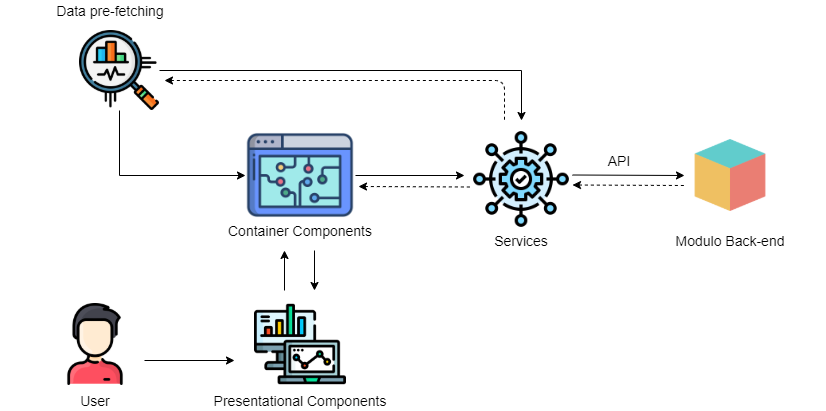
\includegraphics[scale=0.58]{res/Architettura/Frontend/img/general_frontend}\\
\caption{Front-end module general scheme}
\end{figure}


